% chktex-file 36

\section{Implementation}\label{implementation}

This section describes the implementation process. The design highlighted the usage of the dashboard through its personas and scenarios, while the low fidelity mockups gave an early glance at its appearance. At its core, the strength of the application revolves around its extensibility and usability. Therefore, a lot of thought went into choosing the best libraries to provide these features.

First, an overview of the entire application is given, after which we go into more detail. The dashboard consists of two major parts common to web development. The back end is described first. This section explains the reasoning behind the chosen technology stack and the general structure. We also specify the back end structures and REST API calls for each module and component which the front end has access to. For the front end, we explain how the Polymer 3 library supports our modular design and its underlying principles. Hereafter, other libraries used during the implementation, the general front end structure, and the resulting dashboard and its modules are explained. 

It is without question that during the implementation small changes were made to the design. These changes are documented for both parts. During the entire development process, only basic authentication was implemented. The implementation of standards, privacy rules, and security techniques do not contribute towards the goal of the dashboard we defined in the design section. Therefore, we consider these topics out of the scope of the prototype.

    \subsection{Overview}\label{implementation_overview}

    The first major choice that was made, was the type of application to develop: a native application or a web application. It was a relative simple choice, but nonetheless an important one. Native applications are developed, in most cases, for one type of operating system. If a vendor wants to support both Android and iOS devices, two separate applications need to be developed. This requires more developers to not only create the application, but also to maintain it. Another drawback of native applications is the update process. This process often requires the reinstallation of the entire application, which is very disruptive and difficult to do in a care setting.

    Web applications saw a surge in popularity. Compared to their native counterparts, web applications today are becoming increasingly similar in terms of functionality and design. Office Online from Microsoft is a good example showcasing this, which features many functions found on the desktop versions of the Office Suite. While these web applications also require updates, these happen on the server side. When the user refreshes the web page, the latest version of the application is automatically retrieved. This simplifies the roll-out process significantly. Also, all operating systems that support web browsers, are capable of running this type of applications. This includes mobile devices. As a result, developers only have to develop one application. However, the variation in screen resolutions and aspect ratios calls for a responsive design.

    With this in mind, the choice to create a web application was evident. Users can view the dashboard regardless of the device they use, without sacrificing functionality. However, there are also disadvantages to web applications. For example, complex operations will not fit easily into a web application. The strength of web apps also leads to its major drawback: poor performance. A native application can draw much more computational power from the device it was made for. To transfer the computation burden to the server is also not a viable solution as this puts additional strain on the network. In case of real-time applications, latency becomes an issue due to continuous data transfer. However, the dashboard application should not experience any performance issues as the modules that were defined in section~\ref{app_specification} do not require complex operations. Another drawback is that a web applications requires a connection to a web server. However, retrieving medical records require a connection to a data repository anyway, for both web and native applications.

    \begin{figure}[t]
        \centering
        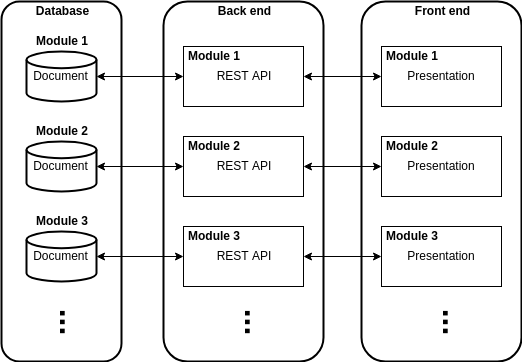
\includegraphics[width=1\textwidth]{chapters/4_implementation/structure}
        \caption{The communication flow by which every module communicates.}\label{fig:structure}
    \end{figure}

    A typical web application consists of two parts: the back end and the front end. In software engineering principles, these refer to the separation of the data access layer and the presentation layer of the web application. For example, the back end fetches data requested by the front end. In turn, the front end presents the retrieved data towards the user. Due to the modular design of the dashboard, each module needs to have its own back and front end structures, visualized by figure~\ref{fig:structure}. As figure~\ref{fig:structure} indicates, there is no direct interaction between the modules, which facilitates low coupling. The next sections describe the back end and front end in detail. Changes made to the design from section~\ref{design} are explained whenever they occur.

    \subsection{Back end}

    \begin{figure}[t]
        \centering
        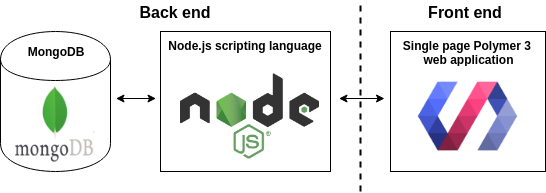
\includegraphics[width=1\textwidth]{chapters/4_implementation/tech}
        \caption{The three core technologies used to build the application.}\label{fig:tech}
    \end{figure}

    The back end is responsible for everything related to the management of the data present in the dashboard application. It is here that the logic is defined to add, update, or remove records from the database based on the requests it received from the front end. The back end exposes a REST API which determines which requests the front end can send.

    This section gives a detailed description of how the back end part of the dashboard was implemented. First, we go over the chosen technology stack after which we explain the back end structure. To close, each component present in the back end is briefly described.

        \subsubsection{Technology stack}

        Figure~\ref{fig:tech} shows the three core technologies used to develop the application. The back end was built using Node.js and MongoDB\@. We now give a brief explanation of what each back end component tries to achieve and why it was chosen.

            \subsubsubsection{Node.js}

            The back end server forms the heart of the dashboard application and Node.js was the preferred choice to implement it. Node.js (or simply Node) is a Java-Script runtime built on Google Chrome's V8 JavaScript engine~\cite{NodeJS}. Node avoids the classic thread-based approach to concurrency, which is relatively inefficient and can be very difficult to use. Instead, it provides concurrency via a single event loop that can support thousands of simultaneous connections, using non-blocking I/O calls. Node also has the added bonus of streamlining web development to the use of a single language.
            
            The main reason Node was chosen, was due to the very large collection of packages that is available through the Node Package Manager (npm). For example, the Express package is only available via Node. This package was of significant help during the entire development process. Also, documentation is easily found thanks to the very large community that develops with Node.

            \subsubsubsection{MongoDB} 
            
            A SQL database is table-based, whereas MongoDB is document-based~\cite{MongoDB}. This type of structure enables highly flexible data schemas, as new data fields can be added without affecting existing documents. This is especially useful when a new data structure from a 3rd party vendor needs to be added to the database. This supports the dashboard's goal of simple extensibility. Also, the developers of MongoDB officially support Node.

            \subsubsubsection{Node packages}

            Node allows developers to easily install a broad selection of packages. We now discuss the packages that were used for the development of the back end. These served many purposes, such as routing, encryption, logging, and request body parsing. 

            \paragraph{Mongoose} Using Node without a library to communicate with MongoDB is very difficult, as data validation and casting must be written manually. By installing Mongoose, a MongoDB object modeling package, this will be taken care of~\cite{Mongoose}. Via this package we can define data schemas and its parameters. Hereafter, a data model is created by compiling the schema. It is now possible to create MongoDB documents in a very similar fashion to object-oriented programming, which encapsulates the more complex inner workings of MongoDB\@. The entire database is constructed via these models.

            \paragraph{Express} Express is a Node web application framework, which helps with the management of routing, connecting middleware, handling requests, and others~\cite{Express}. It can also be of help with organizing a web application on the server side into a MVC architecture. Furthermore, Express makes the creation of a REST API server a much faster process compared to vanilla Node. Since we need to transfer data from MongoDB to our front end via a REST API, this framework is essential. Section~\ref{backend_structure} goes into detail how Express helped define the structure of the back end of the dashboard application.

            \paragraph{Bcrypt \& JSON Web Tokens} Basic encryption is provided by the bcrypt package~\cite{Bcrypt}. Whenever a user registers, the password is hashed and then stored into MongoDB via Mongoose. In case the user successfully authenticates, the JSON Web Tokens package generates a token based on the login name, user id, clearance level, and a secret phrase~\cite{JWT}. This token is sent back to the front end and from now on, must be embed into every future request. After one hour, the token expires and the user must authenticate again.

            \paragraph{Other} The body-parser package helps as its name implies with parsing request bodies. This package is connected to Express as middleware, since it captures the request and parses it before it lands into the developer's hands. For example, accessing parameters in the body of a POST request is done with this simple statement: \texttt{request.body.paramName}. Morgan is another helpful package which logs all requests made to the server. As such, it is a helpful debugging tool. Last, but certainly not least, is the nodemon package. Nodemon detects changes in a Node project. If changes are found, nodemon automatically restarts the server to apply these changes.


        \subsubsection{Structure}\label{backend_structure}
        
        As mentioned before, the Express framework can help with organizing a web application into a MVC architecture. As such, the entire dashboard prototype is built around this architecture. A MVC architecture consists of three parts:
        \begin{itemize}
            \item Model: the part that manages the data and receives input from the controller. This is handled by Mongoose.
            \item View: the view presents the model or in other words, the data. The front end is our view, which is a Polymer 3 server.
            \item Controller: the controller handles incoming requests from the view. Hereafter it calls the model to receive the desired data, which it then returns to the view. This is realized on the back end Node server with the help of Express.
        \end{itemize}

        \noindent Every module present in the back end has three files of the same name that are spread across the following three folders: controller, models, and routes. The following example explains how they are connected:
        \begin{myenumerate}
            \item The front end sends a request to a certain route. Express checks this route and sees that the file \texttt{routes/patient.js} uses it. 
            \item \texttt{routes/patient.js} has every possible API endpoint mapped to a controller function which executes certain logic to retrieve data. All these controller functions are found in the \texttt{controller/patient.js} file.
            \item Last, certain logic gets executed depending on which controller function is called. The controller calls the Mongoose model to perform certain actions on the database, which is defined in \texttt{models/patient.js}.
            \item Depending on the operation, the controller can send data retrieved from the model back to the view. This transaction does not pass by the router.
        \end{myenumerate}

        \noindent In order to extend the dashboard application, these three files need to be created for each component.

        \paragraph{Routing} The routes defined in the back end follow a simple structure. The application starts at the root endpoint: \texttt{/}. Suppose the server receives a request destined for the following endpoint: \texttt{/clinician/login}. At the root level, in \texttt{app.js}, the server forwards all routes starting with ``clinician'' to the routes defined in \texttt{routes/clinician.js}, due to the following line:\\
        \centerline{\texttt{app.use(`/clinician', clinicianRoutes);}}\\ % chktex 36
        All routes defined in \texttt{routes/clinician.js} are therefore called sub-routes, since they aren't defined at the root level.\medskip

        \noindent The same counts for data associated with patients, but one step further. Suppose the server gets the following request: \texttt{/patient/id123/allergy}. The server will forward the \texttt{/id123/allergy} part to \texttt{routes/patient.js}. The patient module will now forward this route to \texttt{/routes/modules/allergy.js}, due to this statement:\\
        \centerline{\texttt{router.use(`/:pId/allergy', allergyRoutes);}} % chktex 36
        
        \subsubsection{Components and dashboard modules}

        We now briefly describe the purpose of every component within the back end of the prototype.

            \paragraph{Clinician} This component allows users to sign up an log in to the system. The controller uses the previously mentioned bcrypt package to provide encryption. Also, the JSON Web Token package is used to return a authentication token should the authentication be successful. The model simply saves the username, encrypted password, and a clearance level. The last field was added to provide basic access control. However, this is not present in the prototype.

            \paragraph{Layout} The layout component allows the front end to save the current configuration of a dashboard. The model stores the patient id, user id, size of the patient info module, a list of the small modules with their corresponding heights and locations, and a list of the main modules with their corresponding dimensions and locations. The existing layout is always deleted first before the new one is saved. This ensures that only one layout configuration exists for every user-patient combination.

            \paragraph{Import} This module makes it possible to import a large set of patient data in a JSON format, which can be useful when migrating to this system. The component calls import functions from the patient component, which is described below. The data needs to be conform to the specification mentioned in appendix~\ref{json_import}.

            \paragraph{Patient} The demographic data of a single patient or of all patients can be requested via this module. The router also receives requests that are meant for the dashboard modules, as explained in section~\ref{backend_structure} during the routing example. The controller also delegates parts of its import process to the relevant modules. For example, if the import information contains a key ``prescriptions'', then the patient controller passes this data on to the prescription controller.

            \paragraph{Dashboard modules} The components related to the dashboard modules are straightforward in terms of functionality. These modules support the CRUD operations. However, the history module only allows the reading of data, since this is sensitive data that should never be deleted. Also, the history controller is called in the other controllers in order to log data changes. Additionally, the telemonitoring has sub-components for each parameter it supports. These are: blood pressure, blood sugar, heart rate, blood oxygen, and weight.

    \subsection{Front end}

    The front end serves as the face of the dashboard application and is more complex than its back end counterpart. Throughout the lengthy implementation phase several changes were made, which required some work to be redone, but in the end promotes better extensibility and usability. 
    
    A modular dashboard was built using the Polymer 3 framework in combination with several libraries. The topics web components and shadow DOM are very important in realizing loosely coupled and highly cohesive modules, which is why it is important to understand them. After the used libraries are explained, the structure of the front end is described. To conclude, the end result is shown via various screenshots of the dashboard and its modules.

        \subsubsection{Polymer 3}

        Polymer is an open-source library that provides a set of feature for creating web components~\cite{Polymer}. The library is developed by Google and contributors. Several Google services such as YouTube and Google Earth were developed with Polymer.

        HTML provides us with standard elements such as \texttt{h1} and \texttt{img}. Web components allow the developer to create custom elements which are used in the same manner as the ones HTML provides. Suppose a calendar web component was created, a developer could add the element to any web page as follows: \texttt{<calendar></calendar>}. The actual definition of the calendar module resides in another file which is imported on the page where it will be used. This approach promotes the creation of reusable components. This also means that the dashboard application can be easily extended with these components. This is largely made possible by the shadow DOM\@.

        \paragraph{Shadow DOM} The Document Object Model describes a tree of documents. The web browser builds such a tree for every web page it loads. The shadow DOM can be seen as a scoped subtree inside a custom element. The root of this subtree is called the shadow root. The structure, styling, and behavior of the children within the shadow DOM do not affect any elements outside of it. Therefore, the appearance and functionality of the custom element is encapsulated and hidden at the document level. Only events fired by elements in the shadow DOM can be caught outside the shadow DOM boundary. This idea of encapsulation is important for our approach towards the dashboard, as each module is responsible for its own appearance and functionality. Developers of custom modules should not need to worry about what happens outside of the shadow DOM\@.

        \subsubsection{Libraries}

        The dashboard must support resizing, and dragging and dropping of modules. To realize this, several libraries were compared with each other and the best fits were chosen. During this section the libraries used to create the front end functionality are described.

            \paragraph{Packery \& Draggabilly} Packery is a JavaScript library that makes gapless and draggable layouts~\cite{Packery}. As items are added and removed from the grid, Packery reorders the layout. The documentation of the library mentions that drag and dropping is supported via the Draggabilly library. This built-in support was the main reason Packery was chosen. There are two Packery grids in the prototype, one for the left panel and one for the main panel. 

            \paragraph{Interact.js} This library implements JavaScript drag and drop, resizing, and multi-touch gestures for modern browsers~\cite{Interact}. However, Draggabilly already provides drag and drop functionality. Since Interact is not supported by Packery, we can't replace Draggabilly with it. Therefore, Interact serves as the library that implements the resizing functionality for the modules.

            \paragraph{Other} The handling of dates throughout the dashboard is done via the Moment library. This library provides very intuitive manipulation methods which are of great help when communicating dates back and forth to the back end. The charts of the telemonitoring are generated via the C3 library, which is a wrapper on top of the D3 library.

        \subsubsection{Structure}

        To start, the entire dashboard is packaged as web component. The application is loaded by placing \texttt{<main-element></main-element>} as the single child in the of the body found in the \texttt{index.html} file. This opens up the ability of having multiple instances of the application open side by side. However, this was not explored further.

        All modules are placed in the \texttt{src} folder. This includes the \texttt{main-element}, but also the following web components: all modules that can be placed on the dashboard, the patient list (\texttt{patient-list-element}), and the patient information module (\texttt{patient-element}). Inside the \texttt{src/modules} folder each module is placed into its own folder. In case the module has both a small and a normal version, two files are found within this directory. Small variants of modules always end with the \texttt{-small} suffix. For example, the allergy module folder contains the files \texttt{allergy-element.js} and \texttt{allergy-element-small.js}.

        The root of the \texttt{src/modules} folder contains the following two files: \texttt{base-
        element.js} and \texttt{base-element-small.js}. These are base web components which all other modules have to extend. This gives each module a streamlined look and design. Also, these base components provide templates which may or must be overridden for the module to work with the dashboard. We describe both base components now in detail.

            \subsubsubsection{Base components}\label{base_components}

            Both base components provide the functions, interface elements, styling, and properties that all modules in the dashboard should have. They serve as a starting point for the developer when creating a new module. It saves the developer time as a basic layout along with utility functions are already defined. They also prevent code duplication. For example, the format of dates displayed in the modules is defined in the base component. Change this format in the base component and it will reflect to all other modules. The next paragraphs go into detail what both the normal and small base components provide.

            \paragraph{Normal base component} The component provides a small block in which a header is defined. This header contains a placeholder title and dialog button. A button in the top right corner to remove the module is also present in the header, which can not be overridden or removed. Five templates exist which can be overridden: 
            \vspace{-6pt}
            \begin{myenumerate}
                \item \texttt{cssTemplate}: define the CSS styling here. Is empty in the base module.
                \item \texttt{ironAjaxTemplate}: define ajax calls here using the \texttt{iron-ajax} web component. Is empty in the base module.
                \item \texttt{dialogTemplate}: define dialogs that may be opened by the module in this template. Is empty in the base module.
                \item \texttt{contentTemplate}: contains the actual content of the module. Contains a placeholder in the base module.
                \item \texttt{dialogButtonTemplate}: specify the action to occur when this button is clicked, such as opening a settings dialog to configure the module. Contains a placeholder in the base module.
            \end{myenumerate}

            \noindent The title can be overridden by modifying the property in the extending module, which the following statement does: \texttt{this.title = `Vaccinations';}\medskip

            \noindent Finally, the base component provides several functions, some of which are placeholders that need to be overridden. These functions serve either as utilities for use within the module, such as getting a formatted date string, or as a function that is called from the \texttt{main-element}, such as getting the minimum size of the module. We now list these functions:
            \vspace{-6pt}
            \begin{myitemize}
                \item \texttt{setDateFormats(datePicker)}: sets the format of the date picker if one is present in the module.
                \item \texttt{getDateString(date)}: converts a date to a string in the DD/MM/YYYY format.
                \item \texttt{getTimeString(date)}: gets the specific time from a date in the HH:mm format.
                \item \texttt{setPatientId()}: stores the id of the current loaded patient to a class variable.
                \item \texttt{update(e)}: called by the \texttt{main-element} to signal that the module should refresh its data. Needs to be overridden to send the data requests to the correct route.
                \item \texttt{sendUpdateSignal()}: should be overridden to fire a signal telling the \texttt{main-element} all instances of this module should refresh their data. The dashboard will do this by calling \texttt{update(e)} from those modules.
                \item \texttt{getMinSizes()}: called by the \texttt{main-element} when creating the module. Should be overridden by returning the minimum width and height of the module.
                \item \texttt{getSettings()}: called by the \texttt{main-element} when saving the module layout. Should be overridden to return the state of the module in case it needs to be saved.
                \item \texttt{loadSettings(settings)}: called by the \texttt{main-element} when loading the layout. Should be overridden in order to restore the state of the module.
            \end{myitemize}

            \paragraph{Small base component} The smaller component is similar to its normal counterpart. However, it is smaller in terms of what it provides. This module also contains a header with a placeholder title. The only other part of this header is the remove button. All templates except the \texttt{dialogButtonTemplate} from the normal base component are present and have the same purpose in the smaller version. The title of this module is also overridden in the same manner as the normal base component. The smaller module provides a subset of the functions of its counterpart:
            \vspace{-6pt}
            \begin{myitemize}
                \item \texttt{getDateString(date)}: converts a date to a string in the DD/MM/YYYY format.
                \item \texttt{setPatientId()}: stores the id of the current loaded patient to a class variable.
                \item \texttt{update(e)}: called by the \texttt{main-element} to signal that the module should refresh its data. Needs to be overridden to send the data requests to the correct route.
                \item \texttt{sendUpdateSignal()}: should be overridden to fire a signal telling the \texttt{main-element} all instances of this module should update their data. The dashboard will do this by calling \texttt{update(e)} from those modules.
                \item \texttt{getMinHeight()}: called by the \texttt{main-element} when creating the module. Should be overridden by returning the minimum height of the module.
                \item \texttt{getSettings()}: called by the \texttt{main-element} when saving the module layout. Should be overridden to return the state of the module in case it needs to be saved.
                \item \texttt{loadSettings(settings)}: called by the \texttt{main-element} when loading the layout. Should be overridden in order to restore the state of the module.
            \end{myitemize}

        \subsubsection{Dashboard}

        Once the user opens the application, Packery will initialize the grids found in the two panels of the dashboard. Hereafter, the user must authenticate by providing his/her credentials. If the authentication succeeded, then the patient list will present itself. If the authentication failed, the user will have to try again. Once a patient is selected, the process of loading the layout starts, which we describe in the next section.

            \subsubsubsection{Layouting}

            \paragraph{Load configuration} As soon as a patient is selected, Packery removes all modules that are present in the two grids. Hereafter, the patient information module is added to the left panel. Now the module configuration can be loaded, which consists of the following steps:
            \vspace{-6pt}
            \begin{myenumerate}
                \item Call the API to receive the layout configuration of the current patient.
                \item Load the small modules:
                \begin{myenumerate}
                    \item Create the module.
                    \item Set the configured height of the module.
                    \item Add the module to the grid of the left panel and tell Packery to place it at the location where it originally was.
                    \item Restore the state of the module by loading its settings.
                \end{myenumerate}
                \item Load the other modules:
                \begin{myenumerate}
                    \item Create the module.
                    \item Set the configured width and height of the module.
                    \item Add the module to the grid of the main panel and tell Packery to place it at the location where it originally was.
                    \item Restore the state of the module by loading its settings.
                \end{myenumerate}
            \end{myenumerate}
            
            \noindent This process only occurs when switching between patients. If there is no configuration, the dashboard will be empty.

            \paragraph{Save configuration} Whenever the user makes changes to the layout of the dashboard, the layout is automatically saved. The auto-save happens after one of the following events occur in either panel: adding or removing a module, moving a module, resizing a module, or changing the state of a module. The save process is as follows:
            \vspace{-6pt}
            \begin{myenumerate}
                \item Retrieve all main modules from Packery and retrieve their settings, and calculate their sizes and locations.
                \item Retrieve all small modules from Packery and retrieve their settings, and calculate their heights and locations.
                \item Retrieve the current size of the patient information module.
                \item Send all this information via the REST API to the back end.
            \end{myenumerate}

            \subsubsubsection{Adding modules} % en drag en drop

            The creation of the modules in itself was not difficult to do. However, an issue arose in an attempt to make these modules draggable. In order to make something draggable with Draggabilly, the library needs to have an identifier of an object such as a class name, that will serve as a drag handle. The original plan was to provide drag and drop by selecting the module title in the header of the module. This would serve as the drag handle. However, Draggabilly could not find the identifier, because it was encapsulated in the shadow DOM of the module.

            The solution to this problem was to place the web component into a container which contains a thin bar at the top that serves as the drag handle. This is automatically done for all modules and does not require extra attention from the developers. Screenshots show the small grey bar at the top of the module. The following steps were taken to create the container:
            \vspace{-6pt}
            \begin{myenumerate}
                \item Create the module and the container.
                \item Set the resize event listeners on the container.
                \item Set the minimum dimensions of the container.
                \item Create the handle with its corresponding class name.
                \item Append the handler to the container.
                \item Append the new module to the container.
                \item Set the remove and broadcast event listeners.
                \item Add the container to the Packery grid.
                \item Create a Draggabilly object for the container and bind it to Packery.
            \end{myenumerate}

            \subsubsubsection{Resizing}

            As mentioned before, the Interact library was used to implement resizable components. For small modules, resizing is only possible by dragging the bottom edge. The normal modules can be resized by dragging the bottom and right edges. In order to provide a clean layout, the modules are resized in chunks of 20 pixels. This simplifies the process of arranging into a neat layout. This was done by subtracting the remainder of the division by 20 of both the width and height during the resize. In case the new width or height is different from the current one, then the resize occurs. While resizing, Packery wil move other modules out of the way. Interact also provides a listener to detect when the resizing has ended. After each resize end, the dashboard saves the layout changes.

        \subsubsection{Modules}

        \begin{figure}[h!]
            \centering
            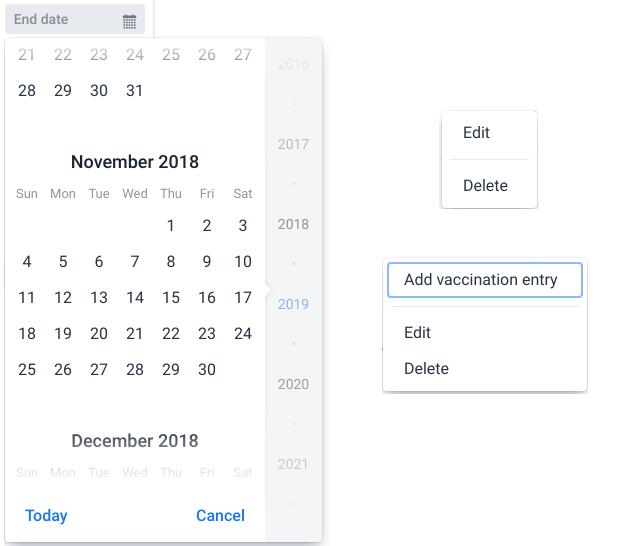
\includegraphics[width=0.8\textwidth]{chapters/4_implementation/vaadin-comps}
            \caption{Left: the \texttt{vaadin-date-picker} component, right: two examples of the \texttt{vaadin-context-menu} component.}\label{fig:vaadin-comps}
        \end{figure}

        This section provides implementation details for each module. Some 3rd party web components were used to provide features needed by several modules. These are the following: \texttt{vaadin-grid}, \texttt{vaadin-date-picker}, and \texttt{vaadin-context-
        menu}~\cite{Vaadin}. We briefly explain what role each Vaadin component has within the dashboard after which we describe the dashboard modules.

        \paragraph{Vaadin grid} The \texttt{vaadin-grid} component creates data tables that have a clear interface and has support to show details of data rows. Throughout the dashboard, all data lists are made with this component.

        \paragraph{Vaadin date picker} This component provides a date selection field. All dates are entered via this component. The user enters dates by either typing them in a correct format, or by selecting the date using the widget, which figure~\ref{fig:vaadin-comps} shows shows on the left.

        \paragraph{Vaadin context menu} The user can press the right mouse button on certain data to delete or update it. Otherwise, buttons would need to be displayed to provide these actions, which may clutter the screen. The data displayed in the Vaadin grid components can be edited this way. Two examples of such context menus are displayed on the right side of figure~\ref{fig:vaadin-comps}.

            \newpage
            \subsubsubsection{Patient list}

            \begin{figure}[t]
                \centering
                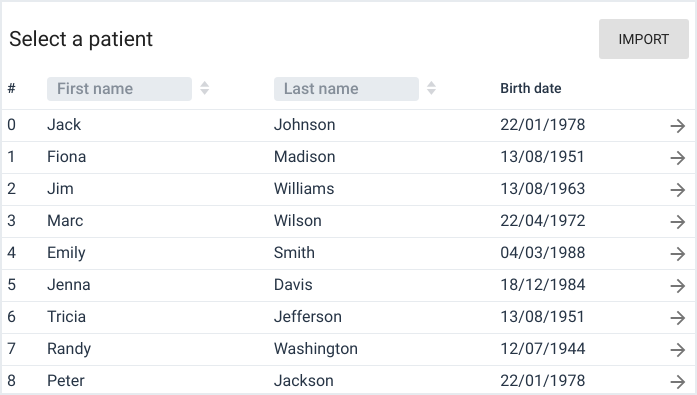
\includegraphics[width=1\textwidth]{chapters/4_implementation/patient-list}
                \caption{The patient list component.}\label{fig:patient-list}
            \end{figure}

            After successful authentication, the user sees the patient list. This list shows basic information concerning the patients that are in the system. Also, it is possible to sort and search by first or last name. As figure~\ref{fig:patient-list} shows, the user can import patients by pressing the button in the top right corner. This opens a dialog box that accepts raw JSON data. The JSON data must follow the specification from appendix~\ref{json_import}. Also, this module does not extend the base component mentioned in section~\ref{base_components} because it will never be placed on the dashboard.

            \newpage
            \subsubsubsection{Patient information}\label{mod_patient_info}

            \begin{figure}[t]
                \centering
                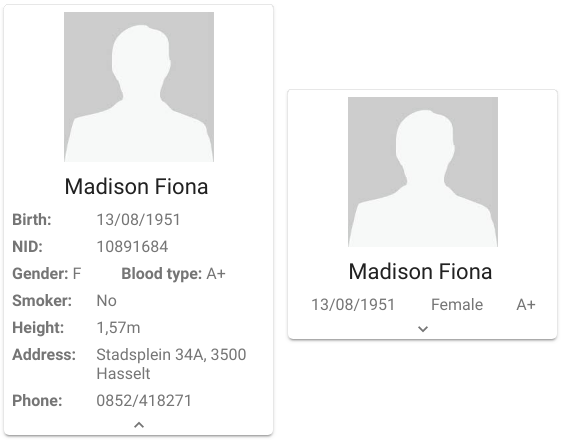
\includegraphics[width=0.8\textwidth]{chapters/4_implementation/patient-info}
                \caption{The two possible sizes of the patient information module.}\label{fig:patient-info}
            \end{figure}

            The patient information module is always present on the left panel of the dashboard and it can not be removed. The reasoning behind this, is that clinicians should always be able to see which dashboard is open. It is possible that the name of the patient only appears in this particular module and if it is removed, confusion may arise. By pressing the arrow button on the bottom, the size of the module changes, which in turn triggers a layout save. Figure~\ref{fig:patient-info} shows the two possible sizes. This was implemented by swapping between two \texttt{div}'s every time the arrow button was pressed. There are no notable changes made to this module, compared to the design. The picture at the top of the module is a placeholder. This module also does not extend the base component, because it can't be freely placed on the dashboard.

            \newpage
            \subsubsubsection{Prescription}\label{mod_prescription}

            \begin{figure}[t]
                \centering
                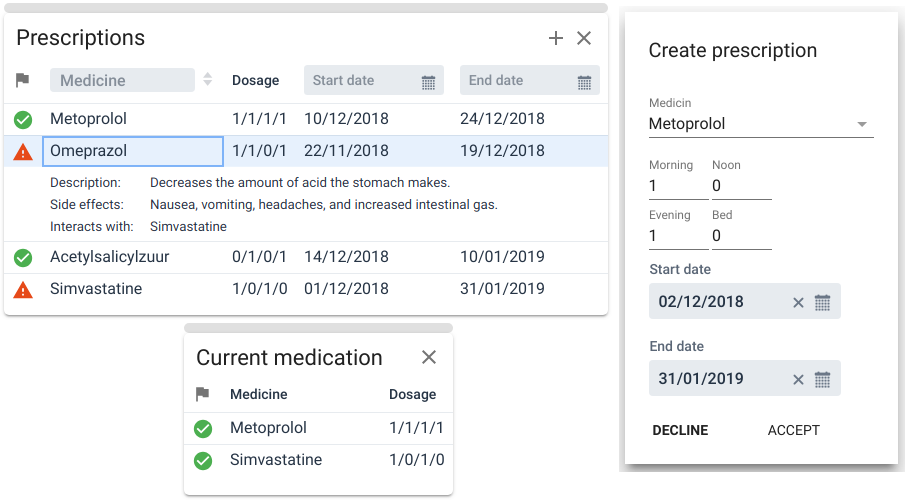
\includegraphics[width=1\textwidth]{chapters/4_implementation/prescriptions}
                \caption{The normal and small version of the prescription module. Adding prescriptions is done via the dialog on the right.}\label{fig:prescriptions}
            \end{figure}

            The prescription module is unchanged compared to the design. This module uses the Vaadin grid for both the small and normal versions to display the prescriptions, as figure~\ref{fig:prescriptions} shows. Removing and editing the prescriptions is done via the Vaadin context menu. Also, note the gray drag handle on top of the modules. In case there are interactions, the icon in the leftmost column changes. Hovering over this icon indicates the interacting medicine.

            When no dates are selected, all prescriptions that were ever assigned to the patient are shown. As soon as two dates are selected, the module checks if they are valid. These checks include that the start date must be before the end date. Every time the module receives prescriptions, it checks for prescriptions against interactions. Because this is a prototype, fictive interactions were created.

            The small module always shows the medication the patient takes of today. This gives the user a way to quickly see the current medication scheme of the patient, without showing too much details. As such, from the small module no prescriptions may be added, edited, or removed.

            \newpage
            \subsubsubsection{Allergy}\label{mod_allergy}

            \begin{figure}[t]
                \centering
                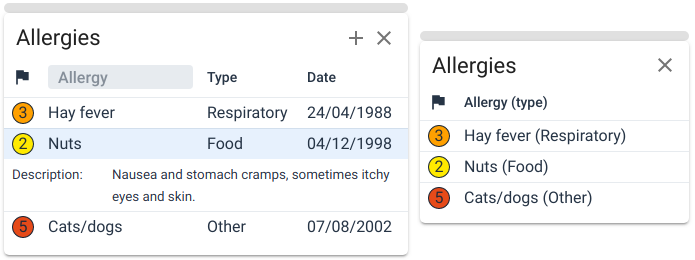
\includegraphics[width=1\textwidth]{chapters/4_implementation/allergies}
                \caption{The normal and small version of the allergy module.}\label{fig:allergies}
            \end{figure}

            The allergy module may be the simplest one in terms of design and functionality, but it still is an important part of an EHR\@. No changes were made to the design of the module. Shown in figure~\ref{fig:allergies}, a more severe reaction to the allergy is indicated by a red icon. Again, the small module only serves as a reference and no changes to the allergies can be made from here.

            \subsubsubsection{Vaccination}\label{mod_vaccination}

            \begin{figure}[t]
                \centering
                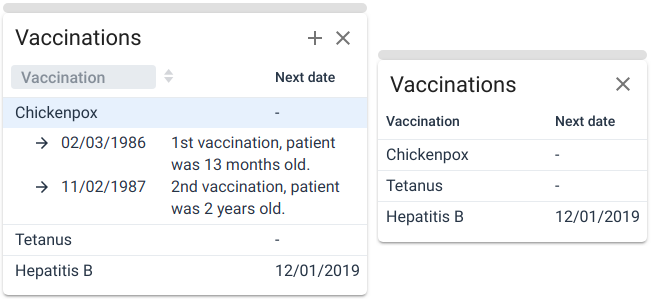
\includegraphics[width=1\textwidth]{chapters/4_implementation/vaccinations}
                \caption{The normal and small version of the vaccination module.}\label{fig:vaccinations}
            \end{figure}

            This module is very similar to the allergy module. It shows a list of conditions for which the patient is vaccinated. In case a revaccination is scheduled, this date is also shown. For each condition, historical vaccinations can be added via the context menu (figure~\ref{fig:vaadin-comps}, right). These vaccination entries have a description and a date, as shown in figure~\ref{fig:vaccinations}.

            \newpage
            \subsubsubsection{Workflow}\label{mod_workflow}

            \begin{figure}[t]
                \centering
                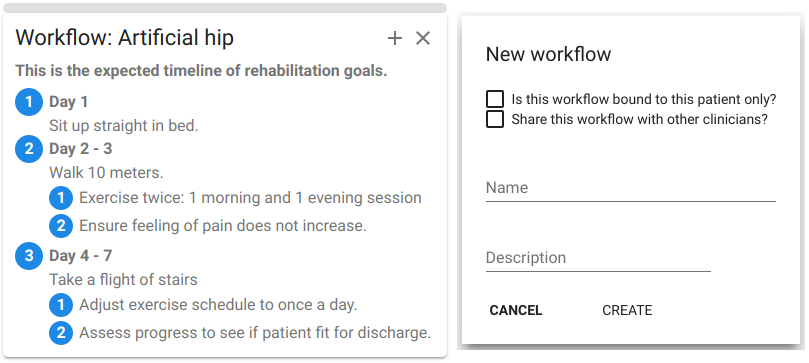
\includegraphics[width=1\textwidth]{chapters/4_implementation/workflow}
                \caption{The workflow module on the left, showing a workflow for the example mentioned in section~\ref{app_specification_modules}. The dialog on the right is used to create a new workflow.}\label{fig:workflow}
            \end{figure}

            The workflow module was difficult to implement. However, there are no significant changes compared to the design. Figure~\ref{fig:workflow} shows a workflow and also the dialog to create a new one. Whenever the user loads a workflow the layout is saved. The module overrides the \texttt{loadSettings(settings)} and \texttt{getSettings()} functions of the base component to save and load the identifier of the currently loaded workflow. It should be noted that multiple instances of this module may be added to the dashboard, with each showing a different procedure. They will not interfere with each other. Because these workflows can contain a lot of information, no small module was made. Providing a summary in this case is not useful, nor clarifying.

            \newpage
            \subsubsubsection{Checklist}\label{mod_checklist}

            \begin{figure}[t]
                \centering
                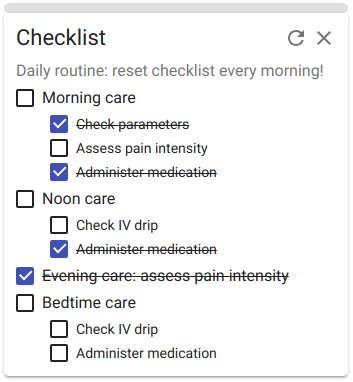
\includegraphics[width=0.5\textwidth]{chapters/4_implementation/checklist}
                \caption{The checklist module.}\label{fig:checklist}
            \end{figure}

            As a result of the workflow module, a new module not mentioned in the design was made. A checklist module was created which allows the user to add tasks and potential sub-tasks. This checklist is bound to the patient, so if one user checks off a task, it will also be checked for another user. The module was implemented by editing a copy of the workflow module, due to being similar in structure. The result is shown in figure~\ref{fig:checklist}. The button to the left of the remove button resets the entire checklist. A small module was not created for the same reasons one wasn't created for the workflow module.

            \newpage
            \subsubsubsection{History}

            \begin{figure}[t]
                \centering
                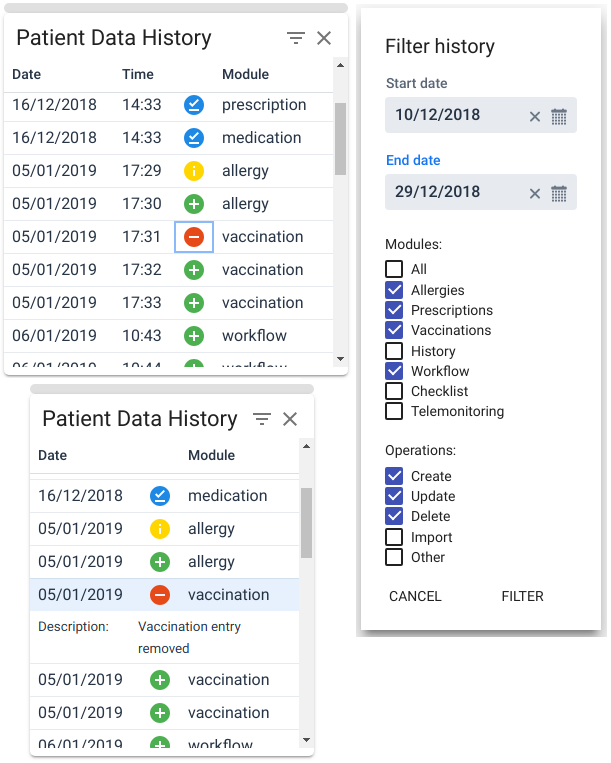
\includegraphics[width=0.8\textwidth]{chapters/4_implementation/history}
                \caption{The history module where the wide module shows an extra column. Filters are set via the dialog on the right.}\label{fig:history}
            \end{figure}

            The history module was added late in development. No significant changes were made to the design. As figure~\ref{fig:history} shows, the wider history module has an extra time column. This was an experiment regarding the resizing functionality to show and hide elements as the component grows or shrinks. Filters are set via the dialog on the right hand side of the figure. Historic entries can not be removed, only read, as they may be examined in an audit. No small module was added, as this can't be summarized in a clear manner. 

            \newpage
            \subsubsubsection{Telemonitoring}\label{mod_tm}

            \begin{figure}[t]
                \centering
                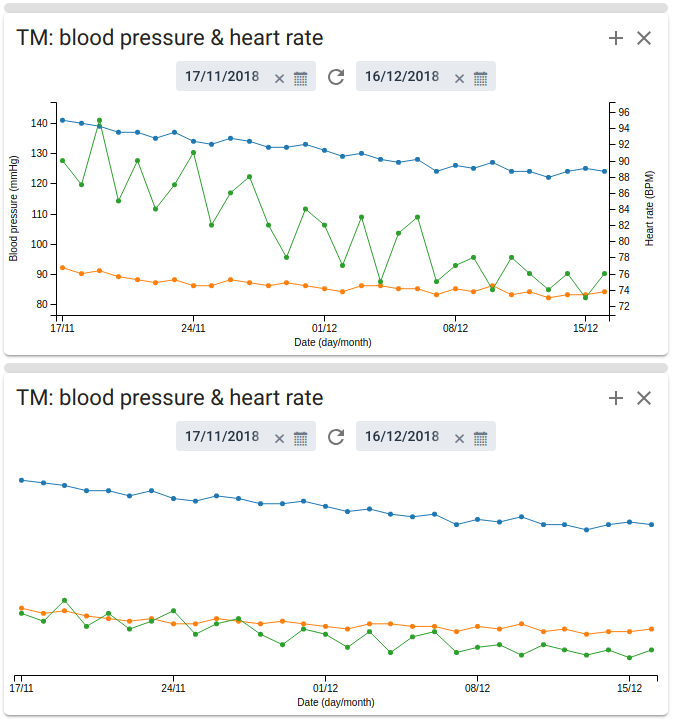
\includegraphics[width=0.8\textwidth]{chapters/4_implementation/tm-compare}
                \caption{The top chart labels both parameters on the y-axis, while the bottom one doesn't.}\label{fig:tm-compare}
            \end{figure}

            The telemonitoring module was the last one to be added to the dashboard. As previously mentioned, C3 was used to plot the data onto a line chart. When the module is added to the dashboard, it will show no data until the user selects the parameters to plot on the chart. This is done by pressing the plus button in the top right corner, which opens a dialog to select the parameters. A maximum of two parameters can be shown on the same chart at a time. In case there are no values for a certain parameter, then the user can't select it. Once a parameter is selected, the user may choose to plot it according to the y-axis. To compare two parameters in relation to each other, it is suggested to plot both these data sets on the y-axis. This normalizes the data on the chart, which in turn makes it easier to compare the data. Figure~\ref{fig:tm-compare} shows the difference. The differences of the green line are in the top chart much more noticeable. However, one can argue that the differences are exaggerated while there is not much difference, which the bottom chart implies.

            Currently, the chart is completely redrawn every time the module changes size. Drawing the chart once and repeatedly resize that one resulted into unexpected behavior where the chart could only grow, but not shrink. Others have reported this on the GitHub page of the library and it is a known issue. As a result the chart is redrawn every time. Thankfully, we did not notice any slowdown. Also, changing the options of the chart will trigger a layout save.

            \begin{figure}[t]
                \centering
                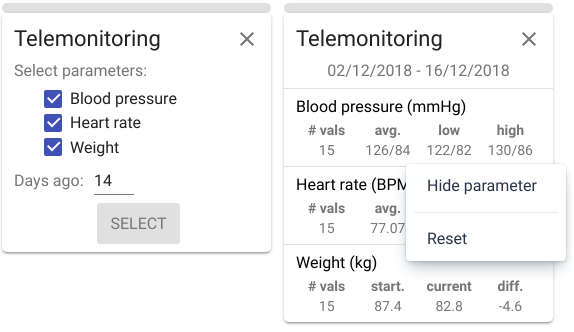
\includegraphics[width=0.7\textwidth]{chapters/4_implementation/tm-small}
                \caption{On the left, the user needs to configure the module. On the right, the summary is shown, together with its context menu.}\label{fig:tm-small}
            \end{figure}

            The small module serves to give a brief summary of all the parameters the user selects for a certain time period. When the module is added, the user must select the parameters to summarize. Also, the user must select a starting date to generate the summary for, by providing the number of days to go back to from today. If the user selects 14, a summary is generated for the data from two weeks ago until today. Once  the module is configured, the layout is saved. To reconfigure the module or hide a parameter, right clicking the parameter will open a context menu. Figure~\ref{fig:tm-small} shows the module. Left on the figure the parameters blood sugar and oxygen are hidden, because there are no data values of those parameters for the current patient. Also, this module can not be resized because the summaries are of fixed height.